\documentclass{beamer}

\title{Data Layout and Compact Representation of BVH Trees for Raytracing}
\author{Андрей Трифонов}

\usetheme{Frankfurt}
\usepackage[main=russian,english]{babel}
\usepackage{xcolor}
\usepackage{algorithm,algorithmic}
\usepackage{graphicx}
\usepackage{hyperref}
\usepackage{listings}
\usepackage{adjustbox}

\begin{document}

\maketitle

\begin{frame}
    \frametitle{References}
    Data Layout:
    \begin{itemize}
        \item
            \href{https://diglib.eg.org/bitstream/handle/10.2312/EGPGV.EGPGV13.057-064/057-064.pdf?sequence=1}
            {\textit{"Analysis of Cache Behavior and Performance of Different BVH Memory
            Layouts for Tracing Incoherent Rays"} by D. Wodniok, A. Schulz, S. Widmer and M. Goese}
        \item
            \href{https://sci-hub.ru/http://dx.doi.org/10.1145/2790060.2790065}
            {\textit{"Bounding Volume Hierarchy Optimization through Agglomerative Treelet Restructuring"}
            by Leonardo R. Domingues and Helio Pedrini}
    \end{itemize}
    Компактное Представление:
    \begin{itemize}
        \item
            \href{https://woizischke.com/ray-tracing-single-slab-hierarchy.pdf}
            {\textit{"Ray Tracing with the Single Slab Hierarchy"}
            by Martin Eisemann, Christian Woizischke and Marcus Magnor}
        \item
            \href{https://diglib.eg.org/bitstream/handle/10.2312/PE.VMV.VMV10.227-234/227-234.pdf}
            {\textit{"The Minimal Bounding Volume Hierarchy"}
            by Pablo Bauszat, Martin Eisemann and Marcus Magnor}
    \end{itemize}
\end{frame}

\begin{frame}
    \frametitle{Что такое BVH?}
    \begin{block}{}
        \textbf{Bounding Volume Hierarchy (BVH)} - иерархия ограничивающих объемов (BV).
    \end{block}
    \begin{figure}
        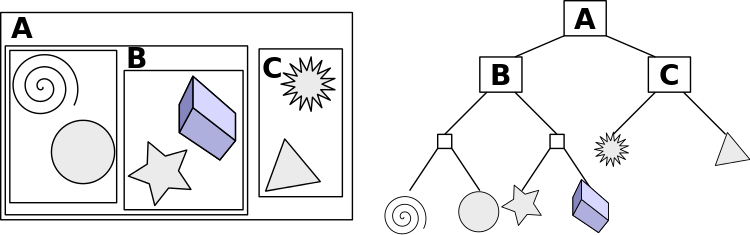
\includegraphics[keepaspectratio, width=\textwidth]{res/bvh.png}
    \end{figure}
    Все геометрические объекты, образующие листовые узлы дерева, заключены в эти BV.

    Затем эти узлы группируются в небольшие наборы и заключаются в более крупные BV.

\end{frame}

\begin{frame}
    \frametitle{Типы BV}
    \textbf{Типы ограничивающих объемов}:
    \begin{itemize}
        \item
            Sphere tree
        \item
            AABB tree (Axis Aligned Bounding Box)
        \item
            OBB tree (Oriented Bounding Box)
        \item
            k-DOP (Discrete Oriented Polytope)
        \item
            SSV (Swept Sphere Volume)
    \end{itemize}
    \begin{figure}
        \begin{center}
            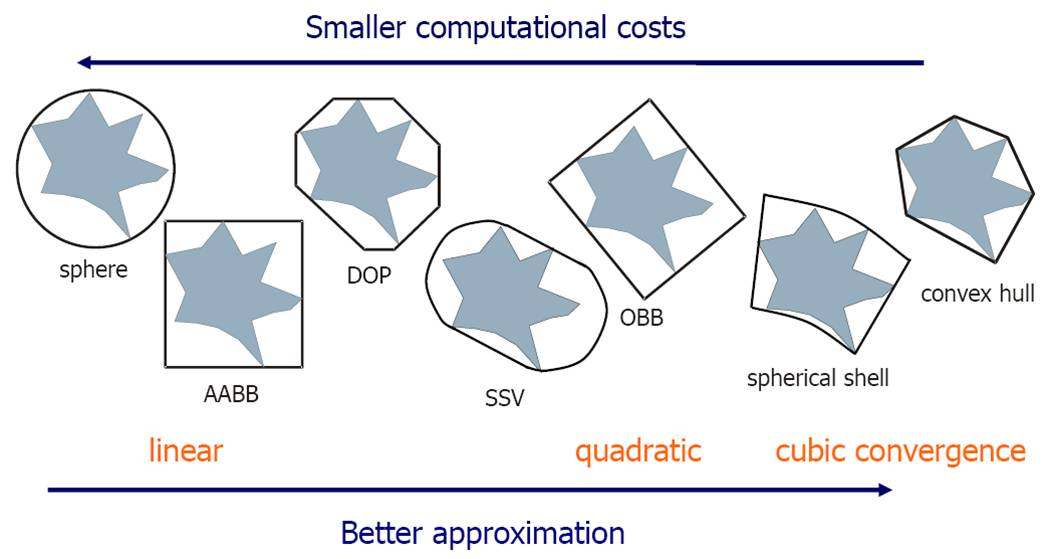
\includegraphics[keepaspectratio, scale=0.3]{res/bvh_types.jpg}
        \end{center}
    \end{figure}
\end{frame}

\begin{frame}
    \frametitle{BVH для трассировки лучей}
    \begin{block}{Зачем?}
        BVH часто используются в трассировке лучей для устранения потенциальных кандидатов
        на пересечение в сцене путем пропуска геометрических объектов,
        расположенных в ограничивающих объемах,
        которые не пересекаются текущим лучом.
    \end{block}
    Путем организации BV в BVH временная сложность (количество выполненных тестов)
    может быть уменьшена с линейной до логарифмической от количества примитивов (треугольников).

    В контексте ускоряющей структуры для рейтрейсинга используются:
    \begin{itemize}
        \item
            AABB (Axis Aligned Bounding Box)
        \item
            OBB (Oriented Bounding Box) \textit{(намного реже)}
    \end{itemize}


\end{frame}

\begin{frame}
    \frametitle{Метрики}
    \textbf{Для оценки эффективности BVH используются метрики}:
    \begin{itemize}
        \item
            Количество обойдённых узлов (NodesCount – NC)
        \item
            Количество обойдённых листьев (LeavesCount – LC)
        \item
            Кол-во арифметических операций проверки пересечения AABB (или др.) с лучом (AOC)
        \item
            Количество тестов луч-треугольник (или кол-во арифметических операций, TC)
        \item
            Количество длинных прыжков в пределах 1 буфера (LongJumpCount – LJC)
        \item
            Объём памяти, прочитанный (BusLoadInBytes – BLB)
        \item
            Leaf Count Variability (LCV)
        \item
            Время на определённом CPU
        \item
            Время на определённом GPU (не для всех)
        \item
            Общий объём памяти на всё дерево
    \end{itemize}
\end{frame}

\begin{frame}
    \frametitle{Функция стоимости BVH дерева}
    \begin{block}{Traversal cost \(c_T\) }
        Средняя стоимость пересечения луча c BV
    \end{block}
    \begin{block}{Intersection cost \(c_I\) }
        Средняя стоимость пересечения луча с примитивом сцены
    \end{block}
    \begin{block}{Conditional probability \(P(N_c\lvert N)\) }
        Условная вероятность пересечения дочернего узла \(N_c\) при пересеченном узле \(N\)
    \end{block}
    \begin{block}{Cost function}
        \(
        c(N) = \begin{cases}
            c_T + \displaystyle \sum_{N_c} P(N_c \lvert N)c(N_c)  \\
            c_I \lvert N \rvert\text{ \textit{(if N is leaf)} }
        \end{cases}
        \)
    \end{block}
\end{frame}

\begin{frame}
    \frametitle{Расположение данных BVH (Data Layout)}
    \begin{block}{Cache locality CPU \& GPU}
        Локальность кеша относится к вероятности того,
        что последовательные операции будут находиться в кеше и,
        следовательно, будут выполняться быстрее.
    \end{block}
    \begin{block}{GPU Texture memory}
        Этот аппаратный блок предоставляет свой механизм кэширования глобальной памяти GPU.
        \begin{itemize}
            \item
                максимизации 2D пространственной локальности
            \item
                аппаратная обработка адресов, выходящих за границы
        \end{itemize}
    \end{block}
    \begin{block}{Data Layout}
        Изменения порядка узлов и их внутреннего представления может улучшить \textbf{cache locality}
        и тем самым уменьшить \textbf{traversal cost}.
    \end{block}
\end{frame}

\begin{frame}[t]
    \frametitle{Clustered Data Layout}
    \framesubtitle{Расположение данных BVH}
    \begin{figure}
        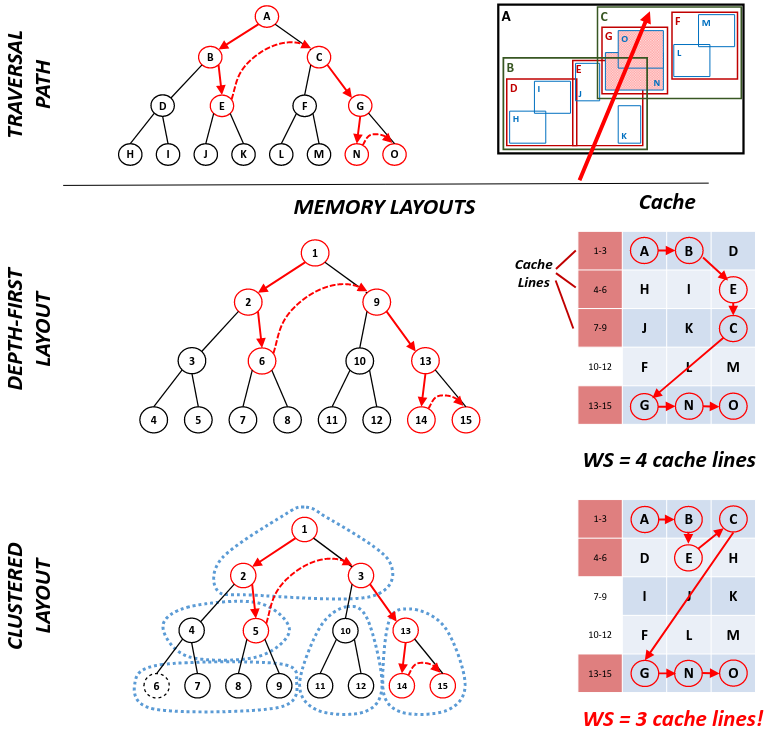
\includegraphics[height=0.75\textheight]{res/clusters.png}
    \end{figure}
\end{frame}

\begin{frame}[t]
    \frametitle{Treelets. Маленькие узлы-деревья}

    \begin{block}{Идея}
        Объеденить близкую друг к другу геометрию в \textbf{узлы-деревья} - \textit{treelets}, чтобы повысить
        \textit{cache locality}, так как следующие когерентные лучи будут попадать в загруженные в \textit{texture memory} трилеты
    \end{block}
    \begin{block}{}
        Поскольку \textbf{время выполнения} и \textbf{требования к памяти} быстро растут вместе с размерами дерева трилета,
        целесообразно использовать только \textit{маленькие древовидные структуры}
    \end{block}
    Перестановкой \textit{treelets} можно уменьшить общюю \textit{SAH cost} \textbf{Treelet BVH (TRBVH)} дерева
\end{frame}

\begin{frame}[fragile]
    \frametitle{Создание трилетов}
    \framesubtitle{Treelets}
    \begin{lstlisting}[language=C++,basicstyle=\ttfamily,keywordstyle=\color{blue}]
    DQ = {root} // deferred queue
    MQ = {} // merge queue
    p = *threshold* // [0; 1]
    while (DQ != {})
        MQ = DQ.pop; ct = {};
        while (MQ != {})
            N = MQ.pop; ct += N
            for (N_c : N)
                if (SAH(N, N_c) > p)
                    if (DFS)
                        MQ.push_front(N_c)
                    else // BFS
                        MQ.push_back(N_c)
        TRBVH += {ct}
    \end{lstlisting}
\end{frame}

\begin{frame}[fragile]
    \frametitle{Agglomerative Treelet Restructuring}
    \begin{lstlisting}[language=C++,basicstyle=\ttfamily,keywordstyle=\color{blue}]
for (internal node i : BVH)
    treelet = FormTreelet(i)
    clusters = treeletLeaves
    while (length(clusters) > 1)
        distances = {}
        for ((x, y) : pairs(clusters))
            d = Dissimilarity(x, y)
            distances = (d, x, y)
        (m, n) = FindMinDistance(distances)
        o = MergeClusters(m, n)
        clusters.remove(m)
        clusters.remove(n)
        clusters.add(o)
    \end{lstlisting}
\end{frame}

\begin{frame}
    \frametitle{Метрика расстояния}
    \framesubtitle{Agglomerative Treelet Restructuring}
    \begin{block}{}
        На каждой итерации пара узлов
        которые ближе друг к другу с использованием данной метрики, будут объединены.
    \end{block}

    \begin{block}{Метрика}
        Поскольку цель состоит в том, чтобы минимизировать общую стоимость SAH дерева,
        за расстояние между двумя кластерами будем считать площадь поверхности
        ограничивающей рамки, содержащей их
    \end{block}

    Это дорогая операция расстояния, поэтому есть смысл кэшировать расстояния между парами кластеров
    заранее 
\end{frame}

\begin{frame}{Треугольная матрица расстояний}
    \framesubtitle{Agglomerative Treelet Restructuring}
    \begin{columns}
        \column{0.5\textwidth}
        Удобно кэшировать расстояния между кластерами в треугольной матрице.

        Рассмотрим измениения в матрице после объединения кластеров 3 и 5
        \begin{block}{Строка и столбец по индексу массива}
            $r = 1 + \lfloor \frac{\sqrt{8i + 1}-1}{2} \rfloor$

            $c = i + \frac{r(r-1)}{2}$
        \end{block}

        \begin{itemize}
            \item 
                Красные - вычислить заново
            \item 
                Синие - скопировать
        \end{itemize}
        \column{0.5\textwidth}
        \begin{figure}
            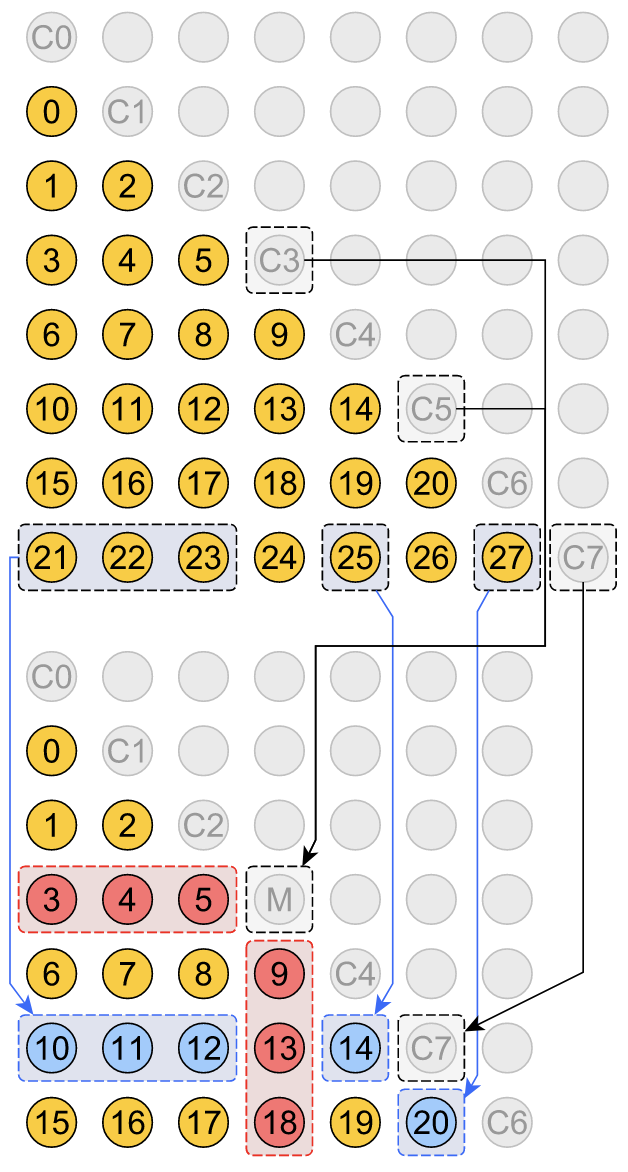
\includegraphics[height=0.75\textheight]{res/dist_matrix.png}
        \end{figure}
    \end{columns}
\end{frame}

\begin{frame}{Объединение кластеров}
    \framesubtitle{Agglomerative Treelet Restructuring}
    \begin{block}{Agglomerative clustering}
        На каждом шаге два кластера, находящиеся ближе друг к другу (по матрице расстояний) объединяются.
        Соединяем объедененные кластеры внутренним узлом (изменяя указатели)
    \end{block}

    \begin{figure}
        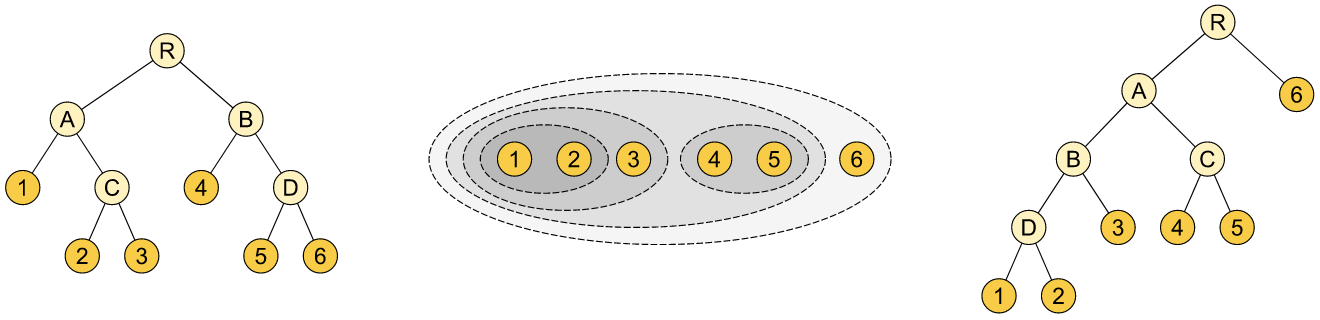
\includegraphics[keepaspectratio, width=\textwidth]{res/merge_treelets.png}
    \end{figure}

    Аллоцировать память на новые узлы не нужно.
\end{frame}

\begin{frame}[t]{SAH cost проверка}
    \framesubtitle{Agglomerative Treelet Restructuring}
    \begin{block}{}
        Все предлагаемые модификации \textbf{сохраняются в списке}, а не применяются сразу
    \end{block}
    Каждая запись списка содержит:
    \begin{itemize}
        \item 
            индекс внутреннего узла, который необходимо изменить
        \item 
            индексы двух его дочерних узлов
    \end{itemize}

    После обработки всего трилета \textit{SAH cost} новой топологии сравнивается
    с первоначальной стоимостью трилета
    \begin{block}{}
        Изменения вступят в силу только в том случае, если стоимость уменьшилась
    \end{block}

\end{frame}

\begin{frame}{Post-processing}
    \framesubtitle{Agglomerative Treelet Restructuring}

    Практика показывает, что \textit{SAH-cost} оптимизированного дерева можно еще уменьшить,
    разрушив (начать хранить примитивы напрямую) некоторые поддеревья

    \begin{block}{Стоимость \textit{разрушенного} дерева}
        \(
        c = c_t A(n) N(n)
        \)

        $n$ - subtree root

        $A()$ - площадь поверхности

        $N()$ - кол-во примитивов (треугольников) в дереве
    \end{block}
    Если полученная стоимость меньше \textit{SAH-cost} поддеревца, то принимаем решение об замене
    поддервца листом с $N(n)$ треугольников
\end{frame}

\begin{frame}{Параметры}
    \framesubtitle{Agglomerative Treelet Restructuring}
    \begin{itemize}
        \item
            размер трилета (кол-во узлов на трилет)

            Оптимальное значение: \textcolor{teal}{9}
        \item
            количество итераций (полные перестроения всей TRBVH)

            Оптимальное значение: \textcolor{teal}{2}
        \item
            $\gamma$ (сколько листьев должно быть в трилете)

            Оптимальное значение: \textcolor{teal}{treelet\_size}, и удваивать на каждой итерации
    \end{itemize}

    \begin{block}{Соотношение скорость качество}
        $\gamma$ определяет может ли узел быть использован в качестве корня трилета.
        Чем больше $\gamma$ тем быстрее скорость конструкции. Уменьшение $\gamma$ приводит к улучшению качества.

    \end{block}

\end{frame}

\begin{frame}[t]{Обход дерева снизу вверх}
    \framesubtitle{Agglomerative Treelet Restructuring}
    Каждый тред начинается с обработки листа.
    \begin{block}{Avoiding race conditions (для бинарного дерева)}
        По умолчанию 2 треда будут достигать каждый узел.
        Введим правило, что за родительский узел берется только второй тред, а первый остается неактивным.
    \end{block}
    Получается при обходе кол-во неактивных тредов в варпе быстро растет.
\end{frame}

\begin{frame}[t]{Память нужная для алгоритма}
    \framesubtitle{Agglomerative Treelet Restructuring}
    В \textit{shared memory} располагаются 3 массива:
    \begin{itemize}
        \item
            \textit{leaf indices}
        \item
            \textit{internal node indices}
        \item
            \textit{leaf surface areas}
    \end{itemize}
    \textit{Leaf surface areas} используются только при формировании трилета, так что этот массив можно использовать для других целей
    при престроении трилета.

    Когда кластеры объединяются, можно использовать последний неиспользуемый узел из \textit{internal node indices} для хранения
    информации в новом кластере.
\end{frame}

\begin{frame}[t]{Занимаемая память}
    \framesubtitle{Agglomerative Treelet Restructuring}
    \textit{52 byte of global memory} на узел:
    \begin{itemize}
        \item
            указатели на родителя и на двух дочерхних узлов
        \item
            индекс
        \item
            площадь поверхности
        \item
            \textit{AABB (32 byte)}
    \end{itemize}
    Прочие траты:
    \begin{itemize}
        \item
            атомарные счетчики
            \textit{(4 byte / node)}
        \item
            кол-во треугольников под узлом
            \textit{(4 byte / node)}
        \item
            \textit{SAH-cost} каждого узла
            \textit{(4 byte / node)}
        \item
            агломеративное расписание (необязательно)
            \textit{(256 byte / treelet size of 32)}
        \item
            матрица расстояний (при размере трилета >21)
            \textit{($\text {number of cluster combinations} * 4 \text{bytes}$ / warp)}

    \end{itemize}

\end{frame}

\begin{frame}[t]{Результаты}
    \framesubtitle{Agglomerative Treelet Restructuring}

    \begin{columns}
        \column{0.8\textwidth}

        \resizebox{\textwidth}{!}{
            \begin{tabular}{|c c c c c c|}
                \multicolumn{6}{c}{Sponza (262K)} \\
                \hline
                Method & Mrays/s & Time & SAH & Memory & Relative \\
                \hline
                LBVH & 56.17 & 7.91 ms & 114.42 & 7 MB & 69.23\% \\
                TRBVH & 81.13 & 37.86 ms & 75.75 & 50 MB & 100.00\% \\
                ATRBVH & 85.99 & 26.43 ms & 75.42 & 12 MB & 105.99\% \\
                ATRBVH* & 77.80 & 30.36 ms & 75.88 & 12 MB & 95.90\% \\
                \hline
        \end{tabular} }

        \resizebox{\textwidth}{!}{
            \begin{tabular}{|c c c c c c|}
                \multicolumn{6}{c}{Hairball (2.9M)} \\
                \hline
                Method & Mrays/s & Time & SAH & Memory & Relative \\
                \hline
                LBVH & 15.33 & 65.71 ms & 541.90 & 77 MB & 92.41\% \\
                TRBVH & 16.59 & 374.22 ms & 478.08 & 520 MB & 100.00\% \\
                ATRBVH & 16.44 & 255.24 ms & 475.72 & 121 MB & 99.10\% \\
                ATRBVH* & 16.44 & 289.69 ms & 477.46 & 121 MB & 99.10\% \\
                \hline
        \end{tabular} }

        \column{0.2\textwidth}
        \begin{figure}
            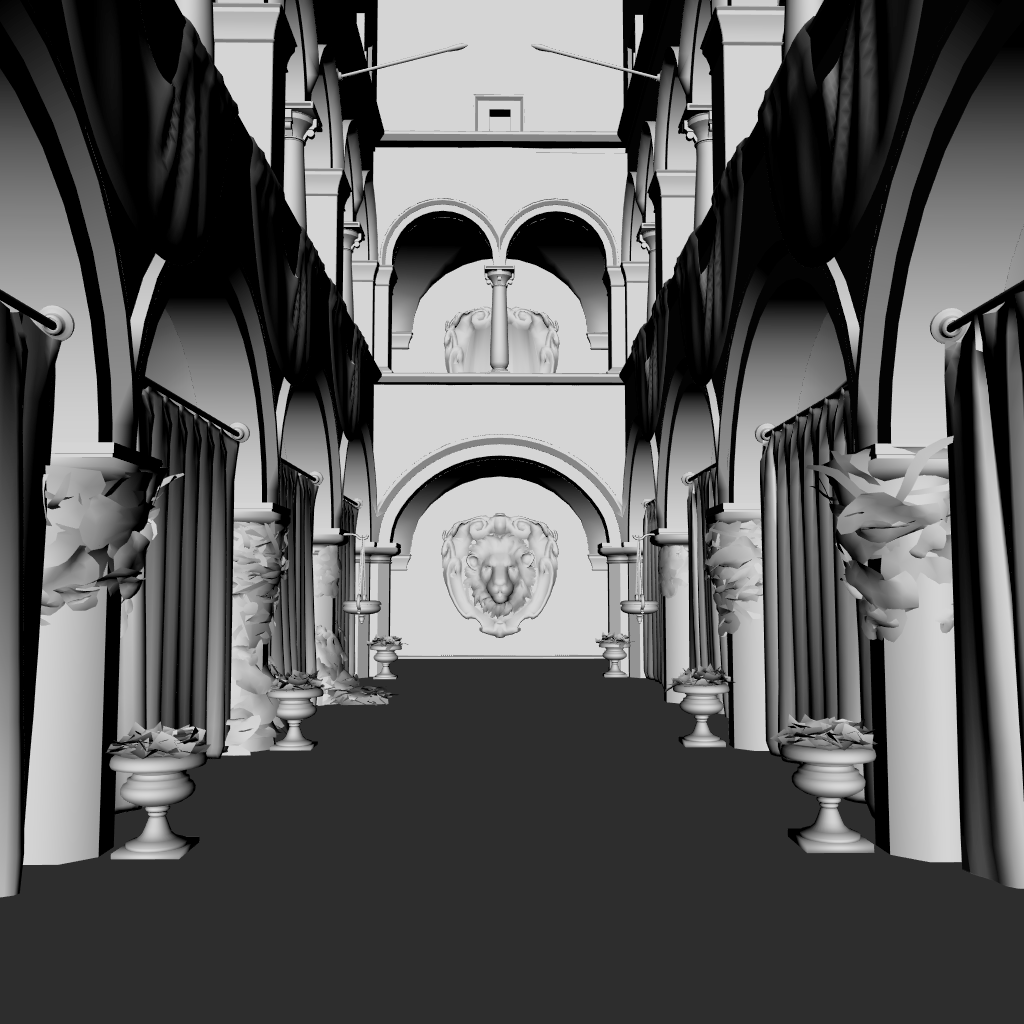
\includegraphics[keepaspectratio, width=\textwidth]{res/sponza.png}
        \end{figure}
        \begin{figure}
            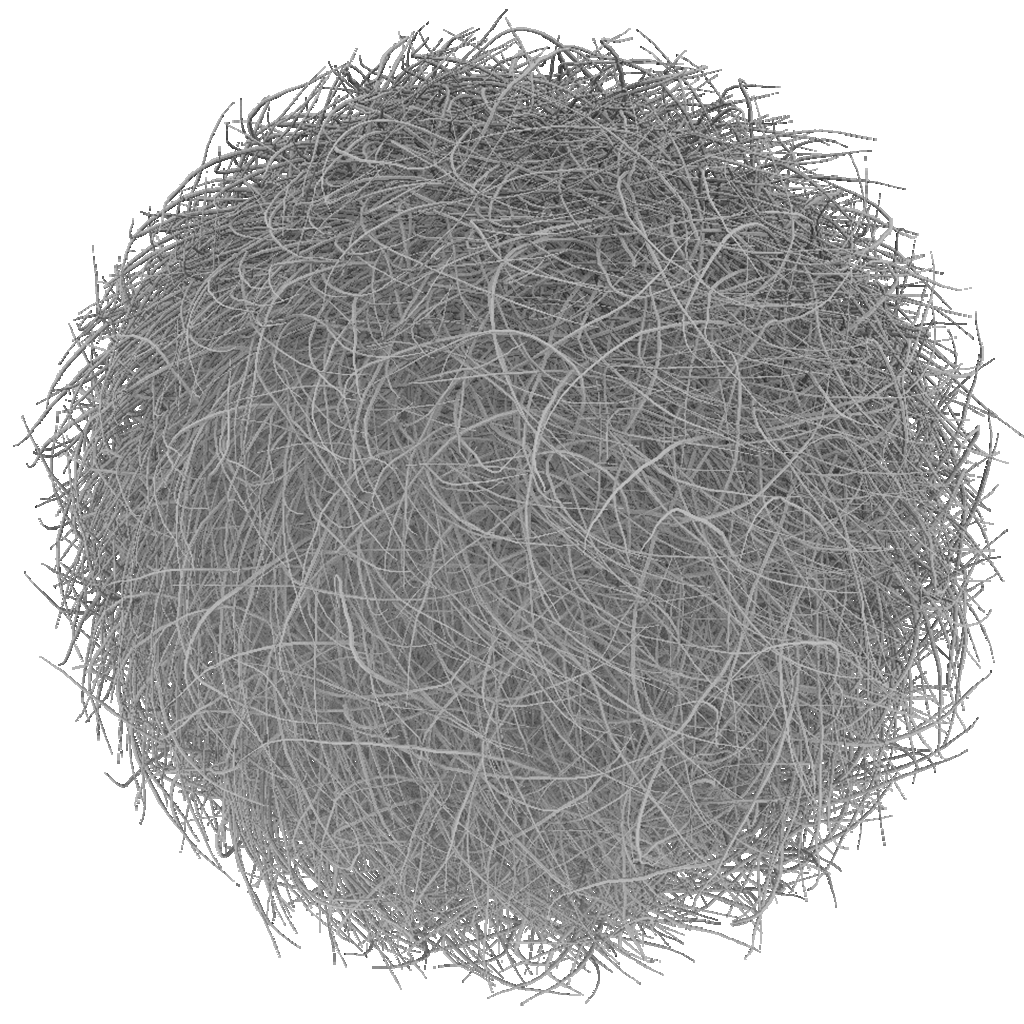
\includegraphics[keepaspectratio, width=\textwidth]{res/hairball.png}
        \end{figure}

    \end{columns}

    \begin{center}
        \resizebox{0.5\textwidth}{!}{
            \begin{tabular}{|c c c|}
                \hline
                Method & Performance (\%) & Time (\%) \\
                \hline
                LBVH & 80.8 & 20.3 \\
                TRBVH & 100 & 100 \\
                ATRBVH & 99.7 & 69.5 \\
                ATRBVH* & 99.9 & 78.4 \\
                \hline
        \end{tabular} }
    \end{center}
\end{frame}

\begin{frame}[t]
    \frametitle{Плюсы и минусы}
    \framesubtitle{Agglomerative Treelet Restructuring}
    \textbf{Достоинства}:
    \begin{itemize}
        \item
            30\% быстрее построение ATRBVH, по сравнению с базовым методом TRBVH (при схожем качестве)
        \item
            Очень параллелизируемый
        \item
            Настраиваемый и гибкий
        \item
            Кол-во необходимой временной памяти сведено к минимуму
    \end{itemize}
    \textbf{Недостатки}:
    \begin{itemize}
        \item
            Параметры не настраиваются динамически
    \end{itemize}
\end{frame}

\begin{frame}{Incremental Traversal}
    \begin{block}{}
        Это техника для повышения эффективности рейтрейсинга путем дешевой арифметики с уменьшенной точностью.
    \end{block}
    Идея заключается в \textbf{последовательном приближении начала луча к пересекаемому узлу}.
    Это и позволяет уменьшить точность для теста пересекаемости луча с плоскостью.
    \begin{block}{}
        Также вычислительные затраты можно уменьшить использую тесты пересечений с родительскими узлами
        \textit{(parent plane sharing)}
    \end{block}
\end{frame}

\begin{frame}{Алгоритм двухуровневой кластеризации}
    \begin{enumerate}
        \setcounter{enumi}{-1}
        \item
            Input: обычное BVH (DFS) \textbf{T} с размером указателей на дочерние узлы размером \textbf{n} бит
        \item
            Из корня дерева \textbf{T} создем адрессные кластеры \textbf{AC} \textit{по COLBVH}
        \item
            Для кадого дочернего \textbf{AC} создем \textit{glue node} \textbf{G}, "склеивая" с родительским узлом, 
            и повторяем \textbf{1}
        \item
            Для каждого \textbf{AC} мы рекурсивно создаем кэш-кластеры \textbf{CC} \textit{по COLBVH}
    \end{enumerate}
    \begin{figure}
        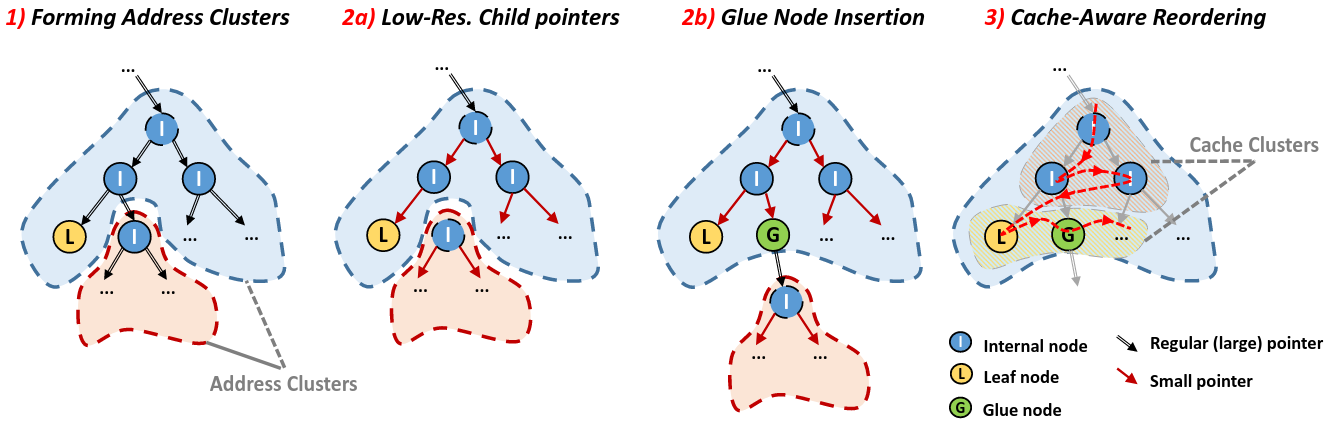
\includegraphics[keepaspectratio, width=\textwidth]{res/2lvl_clustering.png}
    \end{figure}
\end{frame}

\begin{frame}[fragile]{Кластеры адресов. Функция BuildAC}
    \framesubtitle{Двухуровневая кластеризация}
    \begin{lstlisting}[language=C++,basicstyle=\ttfamily,keywordstyle=\color{blue}]
BuildAC(dstOffset, srcRoot) -> offset_t
    maxN = 2^ptr_bits; AC = {}
    child_nodes = {src_root}; child_ACs = {}
    while ((size(AC + children) < maxN)
        && !children.is_empty)
        node = pop_max_SA(child_nodes)
        AC << node
        if (is_internal(node))
            children << node.left << node.right
    for (node : child_nodes)
        if (is_internal(node))
            child_ASs << node << make_glue(node)
        else
            AC << node
    ...
    \end{lstlisting}
\end{frame}

\begin{frame}[fragile]{Кластеры адресов. Функция BuildAC (продолжение)}
    \framesubtitle{Двухуровневая кластеризация}
    \begin{lstlisting}[language=C++,basicstyle=\ttfamily,keywordstyle=\color{blue}]
dst_offset += BUILDCCS(dst_offset, AC)
for (root_node : roots(child_ACs))
    dst_offset = align(dst_offset, cache_layout)
    update_parent_glue_node(root_node)
    dst_offset = BuildAC(dst_offset, root_node)
return dst_offset
    \end{lstlisting}
    \begin{block}{update\_parent\_glue\_node()}
        Офсеты корней дочерних кластеров неизвестны на момент создания склеивающего узла,
        а значит должны быть занесены в \textit{glue nodes} позже
    \end{block}
    \begin{block}{}
        Чтобы шаг кэш-кластеринга имел смысл, нужно чтобы корень каждого \textbf{AC} был
        выровнен по размеру кэш-линии
    \end{block}
\end{frame}

\begin{frame}[fragile]{Кэш-кластеры. Функция BuildCCs}
    \framesubtitle{Двухуровневая кластеризация}
    \begin{adjustbox}{width=\textwidth, keepaspectratio}
        \begin{lstlisting}[language=C++,basicstyle=\ttfamily,keywordstyle=\color{blue}]
BuildCCs(dst_offset, AC) -> offset_t
    maxN = cache_line_size / node_size
    CC_roots = get_root(AC); deferred_CCs = {}
    while (!CC_roots.is_empty)
        child_nodes << CCRoots; CC = {}
        while (size(CC) < maxN && !child_nodes.empty)
            node = pop_max_SA(child_nodes)
            CC << node
            if (is_internal(node))
                childNodes << node.left << node.right
        CC_roots << {childNodes + CCRoots} // DFS
        if (size(CC) == maxN)
            dst_offset = WriteCluster(dst_offset, CC)
        else deferred_CCs << CC
    for (CC : deferred_CCs) // complete but not full
        dst_offset = WriteCluster(dst_offset, CC)
    return dst_offset
    \end{lstlisting}
\end{adjustbox}
\end{frame}

\begin{frame}[fragile]{Кэш-кластеры. Функция WriteCluster}
    \framesubtitle{Двухуровневая кластеризация}
    \begin{block}{}
        Функция \textit{WriteCluster} записывает кэш-кластер в \textbf{BVH}
    \end{block}
    \begin{lstlisting}[language=C++,basicstyle=\ttfamily,keywordstyle=\color{blue}]
WriteCluster(dst_offset, CC) -> offset_t
    update_child_ptr(get_parent(CC[0]));
    for (i in [0; size(CC)])
        dstBVH[dst_offset] = CC[i];
        dst_offset++
    return dst_offset
    \end{lstlisting}
    \begin{block}{update\_child\_ptr()}
        Записать указатели на дочерние узлы, адресс которых мы не знали раньше
    \end{block}
\end{frame}

\begin{frame}[t]{Дальнейшие оптимизации}
    \framesubtitle{Двухуровневая кластеризация}
    \begin{itemize}
        \item
            \textbf{Padding}:
            Кэш-кластер, следующий за неплолным кэш-кластером, стоит хранить с отступом от него -
            так, чтобы начало \textbf{CC} совпадало с началом кэш-линии

            \textit{Нужно следить (ограничивать паддинг), чтобы узлы не выходили за пределы \textit{small pointers}}
        \item
            \textbf{Cluster merging}:
            Можно объединять малетьнькие собранные кластеры, объединяя их узлы и сортируя по SA.
            Чтобы более большие узлы были загружены в кэш-линию
    \end{itemize}
\end{frame}

\begin{frame}[t]
    \frametitle{Компактное представление BVH}
    Существует несколько подходов, которые пытаются \textbf{минимизировать использование памяти}, используя один или несколько из следующих методов:
    \begin{itemize}
        \item
            \textbf{Сокращение информации}, которая хранится для каждого BV
        \item
            \textbf{Снижение точности} данных, которые хранятся в BV
        \item
            Удаление дочерних и примитивных указателей \textbf{неявным индексированием}
        \item
            Повышение коэффициента ветвления (\textbf{числа потомков на узел}), чтобы уменьшить общее количество узлов в BVH
        \item
            \textbf{Сжатие} данных иерархии
    \end{itemize}
\end{frame}

\begin{frame}[t]
    \frametitle{Идеи сокращения информации BVH}

    \begin{columns}
        \column{.8\textwidth}
        \begin{block}{Enclosing Property of BVH}
            Ограничевающее свойство BVH обеспечивает,
            что луч всегда:
            \begin{itemize}
                \item
                    пересекает сначала (или одновременно) узел предок, прежде чем он
                    сможет пересечь дочерние узлы
                \item
                    всегда будет покидать дочерние узлы
                    раньше или одновременно узла-предка
            \end{itemize}
        \end{block}

        \column{.2\textwidth}
        \begin{figure}
            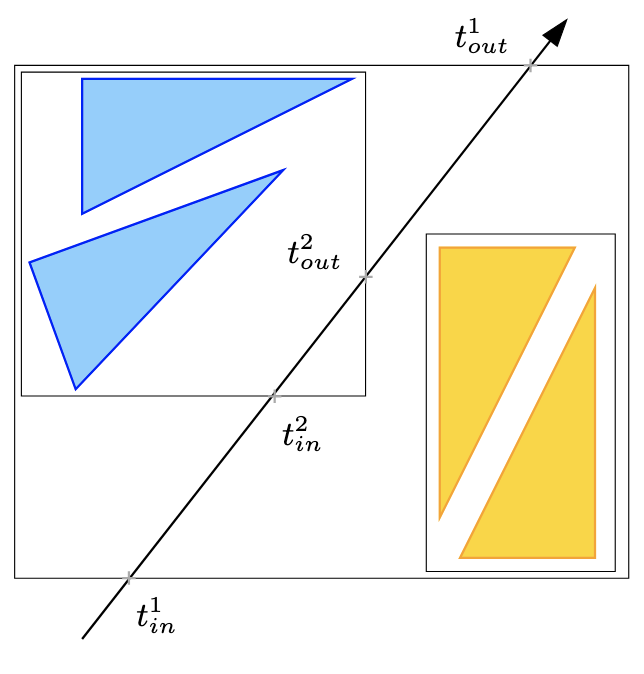
\includegraphics[keepaspectratio, width=\textwidth]{res/enclosing.png}
        \end{figure}
    \end{columns}

    \begin{block}{Еще одно полезное свойство, касающееся эффективности}
        BV дочерних элементов узла имеют общие ограничивающие плоскости со своим родителем.
    \end{block}

\end{frame}

\begin{frame}[t]{Структура узла}
    \framesubtitle{Двухуровневая кластеризация}
    Для имплементации двухуровневой кластеризации было необходимо уменьшить размер узла:
    \begin{itemize}
        \item
            \textbf{Сокращение информации}: \textit{повторное использование плоскостей родительских узлов}

            Для пары дочерних узлов храним 6 плоскостей и \textit{reuse mask}
        \item
            \textbf{Снижение точности}: \textit{квантизация узла}

            Кол-во квантизированных битов определяет компромисс между объемом памяти и качеством BVH

    \end{itemize}

    \begin{figure}
        \begin{center}
            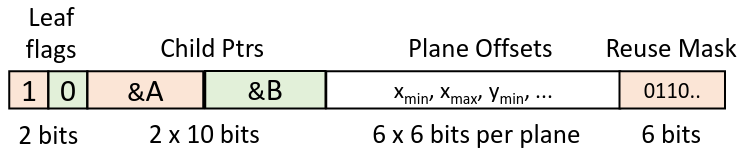
\includegraphics[keepaspectratio, width=\textwidth]{res/8byte_node.png}
        \end{center}
    \end{figure}
\end{frame}

\begin{frame}[t]{Плюсы и минусы}
    \framesubtitle{Двухуровневая кластеризация}
    \begin{itemize}
        \item
    \end{itemize}
\end{frame}

\begin{frame}
    \frametitle{Single Slab Hierarchy}
    \begin{block}{The single slab hierarchy (SSH)}
        \textbf{Иерархия одиночных пластин} - полное k-арное дерево BVH, которое хранится в массиве
        и индексируется как heap.
        Каждый узел либо листовой, либо имеет k дочерних.
        Это способ разделения BV надвое одной пластиной,
        в результате чего получается k-ичное дерево.
    \end{block}

    Принцип, используемый для этого компактного представления BVH:
    \begin{itemize}
        \item
            \textbf{Сокращение информации}, которая хранится для каждого BV
    \end{itemize}

\end{frame}

\begin{frame}
    \frametitle{Bounding Plane Adjustment}
    \framesubtitle{Single Slab Hierarchy}
    Чтобы не оставлять пустот в BVH, для каждого дочернего узла мы подбираем
    свою ось вдоль которой разместить splitting plane (single slab).

    Значит, помимо координаты по оси нашей splitting plane, для каждого узла нужно
    хранить выбранную ось (как флаг).
    \begin{figure}
        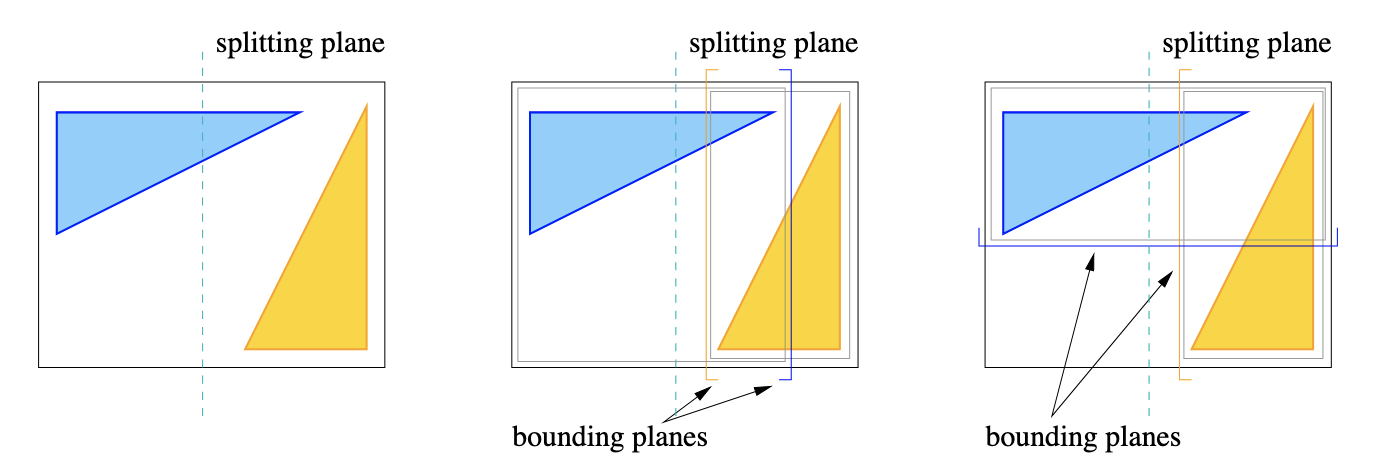
\includegraphics[keepaspectratio, width=\textwidth]{res/splitting_ssh.png}
    \end{figure}
\end{frame}

\begin{frame}[fragile]
    \frametitle{Структура Узла}
    \framesubtitle{Single Slab Hierarchy}

    \begin{semiverbatim}
        #pragma align(8)
        struct SSHNode \{
            float plane;
            union \{
                int firstChildNodeID; //inner nodes
                int firstTriangleID; //leaf nodes
                // bit 0..1: x/y/z/leaf
                // bit 2: left/right interior
                // bit 3..4: traversal axis
            \}
        \};
    \end{semiverbatim}
    Заняв 5 битов флагами у нас остается 27 битов (от int32),
    чтобы сохранить индекс.
    Таким образом можно закодировать до 134 мил. примитивов.

\end{frame}

\begin{frame}[fragile]
    \frametitle{Построение}
    \framesubtitle{Single Slab Hierarchy}

    \begin{lstlisting}[language=C++,basicstyle=\ttfamily,keywordstyle=\color{blue}]
void createSSH(TriangleList tris, AABB parent,
                SSHNode& node) {
    AABB bounds(tris); // bounding box
    float bestSurface = HUGE_VAL;
    int bestSide = 0;
    for (Side side : make_sides(bounds)) {
        AABB temp(parent);
        temp.side = side;
        if (surface(temp) < bestSurface) {
            bestSurface = surface(temp);
            bestSide = side;
        }
    }
    ...

    \end{lstlisting}

\end{frame}

\begin{frame}[fragile]
    \frametitle{Построение (продолжение)}
    \framesubtitle{Single Slab Hierarchy}
    \begin{lstlisting}[language=C++,basicstyle=\ttfamily,keywordstyle=\color{blue}]
    ...
    node.boundingPlane = boudns.bestSide;

    if (tris.size() < n) {
        createLeafNode(); return; }

    TriangleList leftTris, rightTris;
    subdivide(tris, leftTris, rightTris); // SAH
    parent.bestSide = boudns.bestSide;

    int childID = node.firstChildNodeID;
    createSSH(leftTris, parent, childID);
    createSSH(rightTris, parent, childID + 1);
}
    \end{lstlisting}
\end{frame}

\begin{frame}[fragile]
    \frametitle{Обход SSH}
    \framesubtitle{Single Slab Hierarchy}
    \begin{lstlisting}[language=C++,basicstyle=\ttfamily,keywordstyle=\color{blue}]
bool intersectSSH(Ray& ray, mask reverse[3],
        SSHNode* node, float& t_hit,
        float& t_near, float& t_far) {

    // 1. Calculate the distance to its BP
    int axis = node->getSlabAxis();
    float t = (node->plane - ray.origin[axis])
        / ray.dir[axis];
    // 2. Compare it to the active ray segment
    if (node->geometryIsLeft()) {
        t_near = (reverse[axis] | (t <= t_near))
            ? t_near : t;
        t_far  = (reverse[axis] & (t < t_far))
            ? t : t_far;
    ...

    \end{lstlisting}
\end{frame}

\begin{frame}[fragile]
    \frametitle{Обход SSH (продолжение)}
    \framesubtitle{Single Slab Hierarchy}

    \begin{lstlisting}[language=C++,basicstyle=\ttfamily,keywordstyle=\color{blue}]
    ...
    } else {
        t_near = (reverse[axis] & (t > t_near))
            ? t_near : t;
        t_far  = (reverse[axis] | (t >= t_far))
            ? t : t_far;
    }

    if ((t_near > t_far) || (t_near > t_hit)) {
        return false;
    }

    if (node->isLeaf()) { ... } else { ... };
}
    \end{lstlisting}
\end{frame}

\begin{frame}
    \frametitle{Extension to dynamic scenes}
    \framesubtitle{Single Slab Hierarchy}
    \begin{block}{Skinned meshes}
        Можно применить простой bottom-up подход,
        используя тривиальные min/max операции для адаптации границ узлов.
        Структура иерархии остается неизменной.

        Этого достаточно для большинства когерентных анимаций.
    \end{block}

    \begin{block}{Arbitrary movements}
        Можно параллельно перестраивать SSH. Как только построение будет завершено - сделать замену.
    \end{block}

\end{frame}

\begin{frame}[t]
    \frametitle{Плюсы и минусы}
    \framesubtitle{Single Slab Hierarchy}
    \textbf{Достоинства}:
    \begin{itemize}
        \item
            Сжатие 75\%
        \item
            Подходит для интерактивного рейтрейсинга
        \item
            Возможность адаптировать под динамические сцены
        \item
            Более легкий алгоритм траверса (в 6 раз быстрее чем пересекать с AABB)
        \item
            Не изменена структура самого дерева - изменено только представление узлов
        \item
            Сравним по скорости с обычным AABB BVH
    \end{itemize}
    \textbf{Недостатки}:
    \begin{itemize}
        \item
            Немного дольше строить
        \item
            В два раза больше узлов проходит по сравнению с AABB BVH
        \item
            В среднем на один треугольник на луч пересекается больше
    \end{itemize}
\end{frame}

\begin{frame}[t]
    \frametitle{Результаты}
    \framesubtitle{Single Slab Hierarchy}
    \begin{columns}
        \column{0.7\textwidth}
        \begin{itemize}
            \item
                $N_T$: avg of traversed nodes per ray
            \item
                $N_I$: avg of ray-object intersections per ray
            \item
                $T_C$: total time needed for \textbf{construction}
            \item
                $T_R$: total time needed for \textbf{traversal}
            \item
                $s(T_R)$: speedup achieved by the SSH with respect to the BVH
            \item
                $Mem$: memory usage of the AS in megabytes, excluding the triangle data
        \end{itemize}
        \column{0.5\textwidth}
        \begin{figure}
            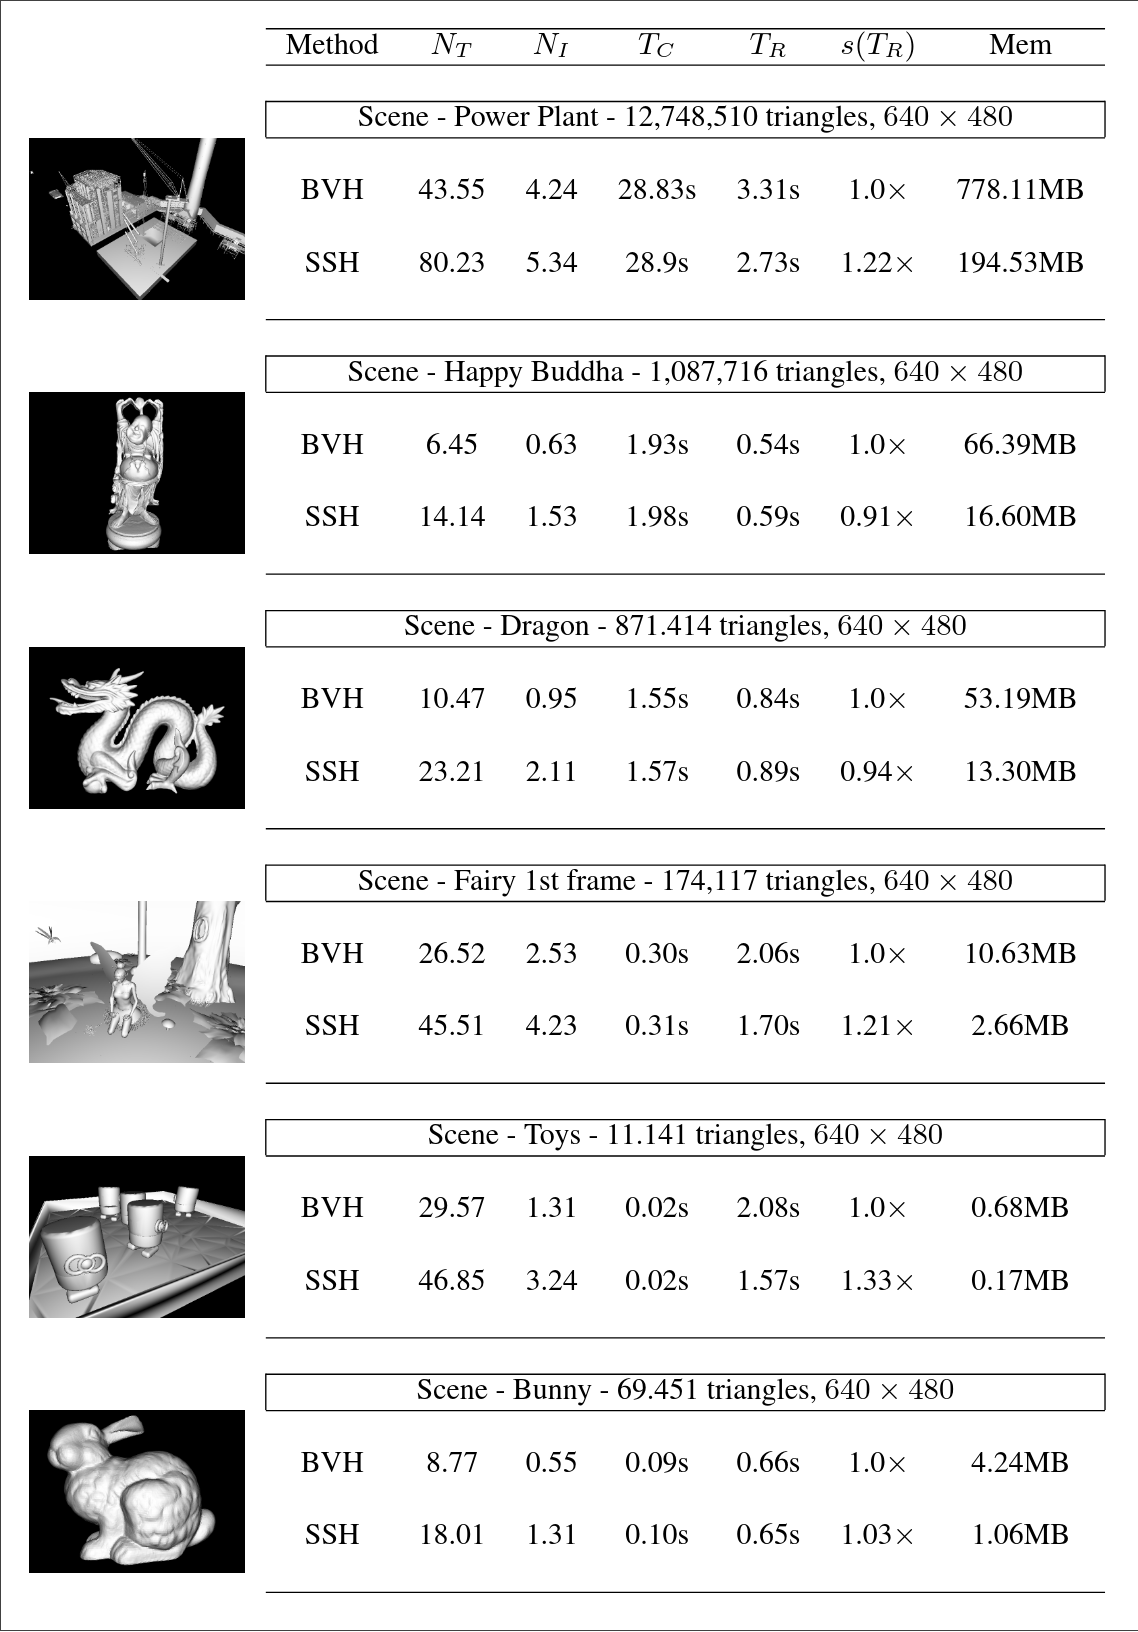
\includegraphics[keepaspectratio, height=.75\textheight]{res/results_ssh.png}
        \end{figure}
    \end{columns}

\end{frame}

\begin{frame}[t]
    \frametitle{The Minimal Bounding Volume Hierarchy}
    \begin{block}{The Minimal Bounding Volume Hierarchy (MVH)}
        Минимальная иерархия ограничевающих объемов - полное k-арное дерево BVH, которое хранится в массиве
        и индексируется как heap.
        Каждый узел либо листовой, либо имеет k дочерних.
    \end{block}
    Принципы, используемые для этого компактного представления BVH:
    \begin{itemize}
        \item
            Удаление дочерних и примитивных указателей \textbf{неявным индексированием}
        \item
            \textbf{Сокращение информации}, которая хранится для каждого BV
    \end{itemize}

\end{frame}

\begin{frame}[t]
    \frametitle{Неявное индексировние}
    \framesubtitle{Minimal Bounding Volume Hierarchy}

    \begin{columns}
        \column{0.5\textwidth}
        \begin{block}{}
            Индексы дочерних узлов $i$-ого узла между $i*k+1$ и $i*k + k$
        \end{block}

        В статье-источнике $k=2$, то есть дерево - бинарное.

        Обозначим кол-во примитивов на узел $n$. И пусть листовые узлы начинаются с индекса $l$.

        \begin{block}{}
            $primID = (i - l) * n$ - будет индекс первого примитива в массиве примитивов для $i$-го узла (если он листовой, то $i > l$).
        \end{block}
        \column{0.5\textwidth}
        \begin{figure}
            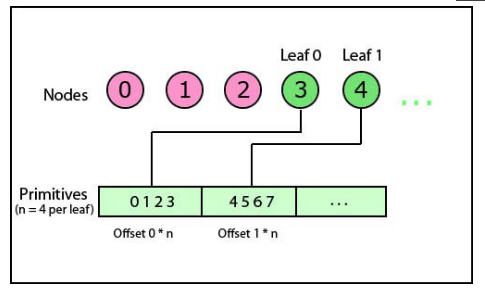
\includegraphics[keepaspectratio, width=\textwidth]{res/mem_layout_mvh.png}
        \end{figure}
        \begin{figure}
            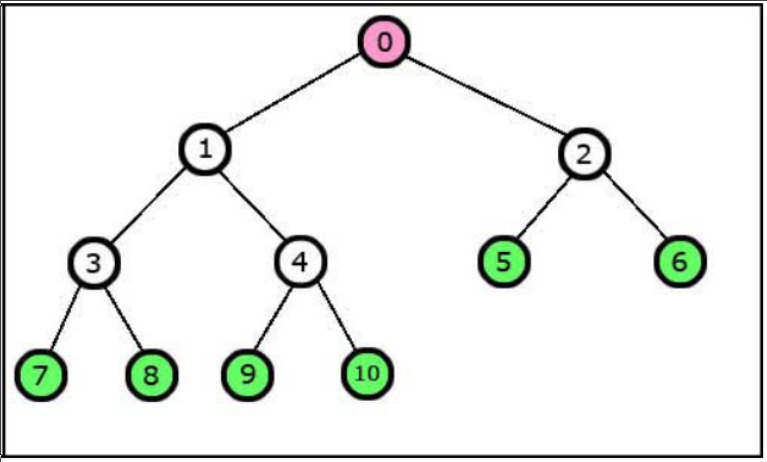
\includegraphics[keepaspectratio, width=0.9\textwidth]{res/tree_mvh.png}
        \end{figure}
    \end{columns}

\end{frame}

\begin{frame}[t]
    \frametitle{Сокращение хранимых данных для узла MVH}
    \framesubtitle{Minimal Bounding Volume Hierarchy}
    \begin{columns}
        \column{0.7\textwidth}
        Выделим для узла всего 2 бита. Получим 4 возможных варианта для получившегося дочернего узла:
        \begin{itemize}
            \item
                No-Cut: if no surface reduction is possible for this node
            \item
                Left-Cut: if the minimum slab is increased
            \item
                Right-Cut: if the maximum slab is decreased
            \item
                Both-Cut: if the Left-Cut and Right-Cut is used
        \end{itemize}
        \column{0.3\textwidth}
        \begin{figure}
            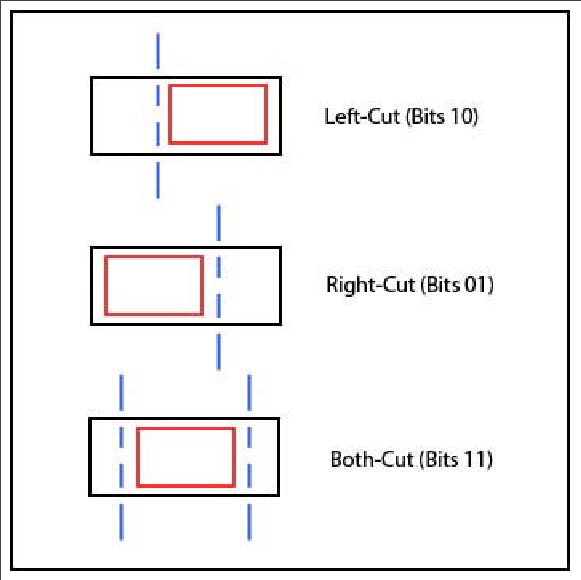
\includegraphics[keepaspectratio, width=\textwidth]{res/splitting_mvh.png}
        \end{figure}
    \end{columns}
    \begin{block}{}
        Каждый раз мы используем фиксированный reduction factor $\zeta$
        Лучшие результаты с $\zeta \in [ 0.35, 0.30]$
    \end{block}

\end{frame}

\begin{frame}
    \frametitle{Построение MVH. Алгоритм}
    \framesubtitle{Minimal Bounding Volume Hierarchy}
    \begin{enumerate}
        \item
            Дублируем последний примитив пока $P$ не станет $ P \% n = 0$
        \item
            Сколько узлов всего? Для $k = 2$ кол-во узлов $2(P/n) -1$
        \item
            Сколько узлов в каждом поддереве?
            \begin{itemize}
                \item[$-$]
                    Присваиваем всем листьям их кол-во примитивов
                \item[$-$]
                    Суммируем bottom-up, пока не дойдем до корня
            \end{itemize}
        \item
            Пусть всего $N$ узлов. Тогда аллоцируем массив длины $2N$ из \textit{int32}
        \item
            MVH строится с использованием object median split, где
            \textbf{процесс разделения} использует предварительно вычисленные количества примитивов для
            разделения списка объектов на две части
    \end{enumerate}
\end{frame}

\begin{frame}
    \frametitle{Процесс разделения BV}
    \framesubtitle{Minimal Bounding Volume Hierarchy}
    \begin{enumerate}
        \item
            Отсекаем от рамки родителя способами 01, 10, 11 и сравниваем с реальным BV для текущего списка примитивов
        \item
            Если один из способов нам подходит - записываем в массив эти 2 бита.
        \item
            Как только дошли до листа - заносим примитивы в массив примитивов под соответствующими индексами
    \end{enumerate}
    \begin{block}{}
        На каждом этапе разделения выбирается ось, вдоль которой располагаются самые длинные грани приближенного AABB
    \end{block}
    \begin{block}{Глобальные параметры}
        \begin{itemize}
            \item
                Root's BB
            \item
                Reduction factor $\zeta$
        \end{itemize}
    \end{block}
\end{frame}

\begin{frame}[fragile]
    \frametitle{Обход MVH}
    \framesubtitle{Minimal Bounding Volume Hierarchy}

    Алгоритм обхода такой же, как и для Single Slab, однако строить splitting plane приходится на самом этапе обхода.

    \begin{lstlisting}[language=C++,basicstyle=\ttfamily,keywordstyle=\color{blue}]
float minTab[4] = { 0.0f, zeta, 0.0f, zeta };
float maxTab[4] = { 0.0f, 0.0f, zeta, zeta };
bool intersect(Ray& r, float& tHit, int* mvhArray,
        int node, AABB& parent,
        float tNear, float tFar) {
    // reconstruct AABB
    vec3 size = parent.max - parent.min;
    char axis = GetAxisOfMaximumExtent(size);
    char bitID = GetNodeCut(node);
    parent.min[axis] += size[axis]*minTab[bitID];
    parent.max[axis] -= size[axis]*maxTab[bitID];

    ...
    \end{lstlisting}

\end{frame}

\begin{frame}[fragile]
    \frametitle{Обход MVH (продолжение)}
    \framesubtitle{Minimal Bounding Volume Hierarchy}

    \begin{lstlisting}[language=C++,basicstyle=\ttfamily,keywordstyle=\color{blue}]
    ...
    // intersection
    float tmin, tmax;
    parent.intersect(r, tmin, tmax, axis);
    float tNear = max(min(tmin, tmax), tNear);
    float tFar = min(max(tmin, tmax), tFar);
    return ((tNear <= tFar) && (tNear <= tHit));
}

char GetNodeCut(int node, int* mvhArray) {
    int iIndex = node >> 4;
    int iShift = (node & 15) << 1;
    return ((mvhArray[iIndex] >> iShift) & 0x3);
}
    \end{lstlisting}

\end{frame}

\begin{frame}[t]
    \frametitle{Двухуровневая MVH. TLAS и BLAS}
    \framesubtitle{Minimal Bounding Volume Hierarchy}
    \begin{block}{Идея}
        \begin{itemize}
            \item
                Половина всех затрат памяти приходится на последний уровень дерева BVH (вдвое больше узлов)
            \item
                Большинство лучей пересакают верхние уровни дерева - надо сделать их качественными
        \end{itemize}
    \end{block}
    \begin{block}{Top level acceleration structure (TLAS)}
        Верхний уровень в несжатом BVH формате, оптимизированный с помощью затратного по времени SAH
    \end{block}
    \begin{block}{Bottom level acceleration structure (BLAS)}
        Нижний уровень состоит из разных MVH, на которые ссылается верхний уровень как на листья.
    \end{block}
\end{frame}

\begin{frame}[t]
    \frametitle{Результаты}
    \framesubtitle{Minimal Bounding Volume Hierarchy}
    \resizebox{\textwidth}{!}{\begin{tabular}{l||l l||l l||l l}
            \hline
            Scene & Tris & BVH & MVH & Ratio BVH:MVH & 2-level MVH & Ratio BVH:2-level MVH \\
            \hline
            Bones & 4,204 & 70.75KB & 0.51KB & 100:1 & 26.59KB & 3:1 \\
            Sponza & 67,462 & 797.94KB & 8.23KB & 97:1 & 41.02KB & 20:1 \\
            Office & 385,376 & 1,636.50KB & 47.04KB & 35:1 & 72.71KB & 23:1 \\
            Fairy & 174,117 & 1,957KB & 21.25KB & 92:1 & 50.41KB & 39:1 \\
            Cars & 549,662 & 6,051.63KB & 67.09KB & 90:1 & 170.20KB & 36:1 \\
            Dragon & 871.306 & 10.44MB & 0.11MB & 101:1 & 142.08KB & 75:1 \\
            Buddha & 1,087,716 & 13.39MB & 0.13MB & 101:1 & 168.50KB & 81:1 \\
            \hline
    \end{tabular} }
    \resizebox{\textwidth}{!}{\begin{tabular}{l||l l l||l l l l l||l l l l l}
            \hline
                  & ts & tt & rt & ts & tt & rt & $\zeta$ & Loss & ts & tt & rt & $\zeta$ & Loss \\
                  \hline
            Bones & 2.5 & 1.3 & 0.10s & 67.7 & 84.3 & 2.70s & 0.3 & 1:27 & 3.2 & 2.7 & 0.16s & 0.3 & 1:1.6 \\
            Sponza & 39.2 & 16.7 & 0.98s & 3,828 & 415 & 160.7s & 0.3 & 1:164 & 159 & 196.6 & 7.35s & 0.3 & 1:7.5 \\
            Office & 26.1 & 63.3 & 1.42s & 1,992 & 262 & 328.2s & 0.4 & 1:231 & 110 & 153.6 & 5.11s & 0.4 & 1:3.6 \\
            Fairy & 21.0 & 10.5 & 0.56s & 12,690 & 3,740 & 519.0s & 0.35 & 1:926 & 72.4 & 83.9 & 3.46s & 0.35 & 1:6.1 \\
            Cars & 44.5 & 15.4 & 1.06s & 4,461 & 1,943 & 221.0s & 0.4 & 1:208 & 148.9 & 186.4 & 7.07s & 0.4 & 1:6.5 \\
            Dragon & 19.3 & 6.6 & 0.51s & 2,081 & 1,676 & 66.8s & 0.35 & 1:131 & 154.1 & 188.0 & 8.04s & 0.35 & 1:15.7 \\
            Buddha & 2.5 & 0.76 & 0.11s & 311 & 262 & 10.37s & 0.35 & 1:94 & 23.3 & 28.4 & 1.27s & 0.35 & 1:11.5 \\
            \hline
            Bones & 19.1 & 219 & 0.02s & 316.4 & 369.9 & 0.06s & 0.3 & 1:3 & 24.6 & 256.6 & 0.02s & 0.3 & 1:1.09 \\
            Sponza & 190.8 & 22 & 0.08s & 1,542 & 3,393 & 1.87s & 0.3 & 1:25 & 784.6 & 2,102 & 0.13s & 0.3 & 1:1.71 \\
            Office & 179.2 & 2,961 & 0.10s & 25,002 & 7,895 & 3.26s & 0.4 & 1:33 & 702.5 & 6,464 & 0.17s & 0.4 & 1:1.74 \\
            Fairy & 185.6 & 2,337 & 0.08s & 49,250 & 8,114 & 3.83s & 0.35 & 1:46 & 683.9 & 5,527 & 0.17s & 0.35 & 1:1.98 \\
            Cars & 332.9 & 2,671 & 0.12s & 20,458 & 14,350 & 2.36s & 0.4 & 1:20 & 1,067 & 6,996 & 0.23s & 0.4 & 1:1.96 \\
            Dragon & 391.0 & 4,399 & 0.15s & 11,244 & 19,142 & 1.55s & 0.35 & 1:11 & 1,777 & 15,468 & 0.40s & 0.35 & 1:2.71 \\
            Buddha & 281.3 & 1,191 & 0.10s & 3,042 & 20,939 & 0.58S & 0.35 & 1:6 & 882.6 & 11,155 & 0.25s & 0.35 & 1:2.38 \\
            \hline
    \end{tabular} }
\end{frame}

\begin{frame}[t]
    \frametitle{Плюсы и минусы}
    \framesubtitle{Minimal Bounding Volume Hierarchy}

    \textbf{Достоинства}:
    \begin{itemize}
        \item
            100:1, 30:1 compression ratio для MVH и двухуровневого решения соотв.
        \item
            Подходит для интерактивного рейтрейсинга
        \item
            Подходит для неимоверно больших сцен
        \item
            Подходит для интерактивного рейтрейсинга (двухуровневая реализация только если)
        \item
            Настраиваемый компромисс между объемом дерева и скоростью
    \end{itemize}

    \textbf{Недостатки}:
    \begin{itemize}
        \item
            Немного дольше строить
        \item
            Сильно страдает от некогерентных лучей
    \end{itemize}

\end{frame}

\end{document}
